% Preamble
\documentclass[a4paper, 12pt]{article}
\usepackage[margin=1in]{geometry} % Set margin
\usepackage{pdfpages} % Insert pdf pages
\usepackage{amssymb,amsmath,amsthm, amsfonts} % Math libraries

% Custom commands
\newcommand{\sub}[1]{\subsection{\underline{#1}}}
\newcommand{\subsub}[1]{\subsubsection{\underline{#1}}}
\newcommand{\R}{\ensuremath{\mathbb{R}}}
\newcommand{\F}{\ensuremath{\mathbb{F}}}
\newcommand{\N}{\ensuremath{\mathbb{N}}}
\newcommand{\Onef}{\ensuremath{1_{\F}}}
\newcommand{\Zerof}{\ensuremath{0_{\F}}}
\newcommand{\eqbcuz}[1]{\text{~$\stackrel{(#1)}{=}$~}}
\newcommand{\eq}[1]{\begin{align*}#1\end{align*}}
\newcommand{\eqn}[1]{\begin{align}#1\end{align}}
\newcommand{\set}[1]{\big{\{} #1 \big{\}}}
\newcommand{\bigset}[1]{\bigg{\{} #1 \bigg{\}}}
\renewcommand{\qed}{\hfill\(\qedsymbol\)}
\newtheorem{lemma}{Lemma}

% Begin Document %
\begin{document}

% Title Page
\begin{titlepage}
    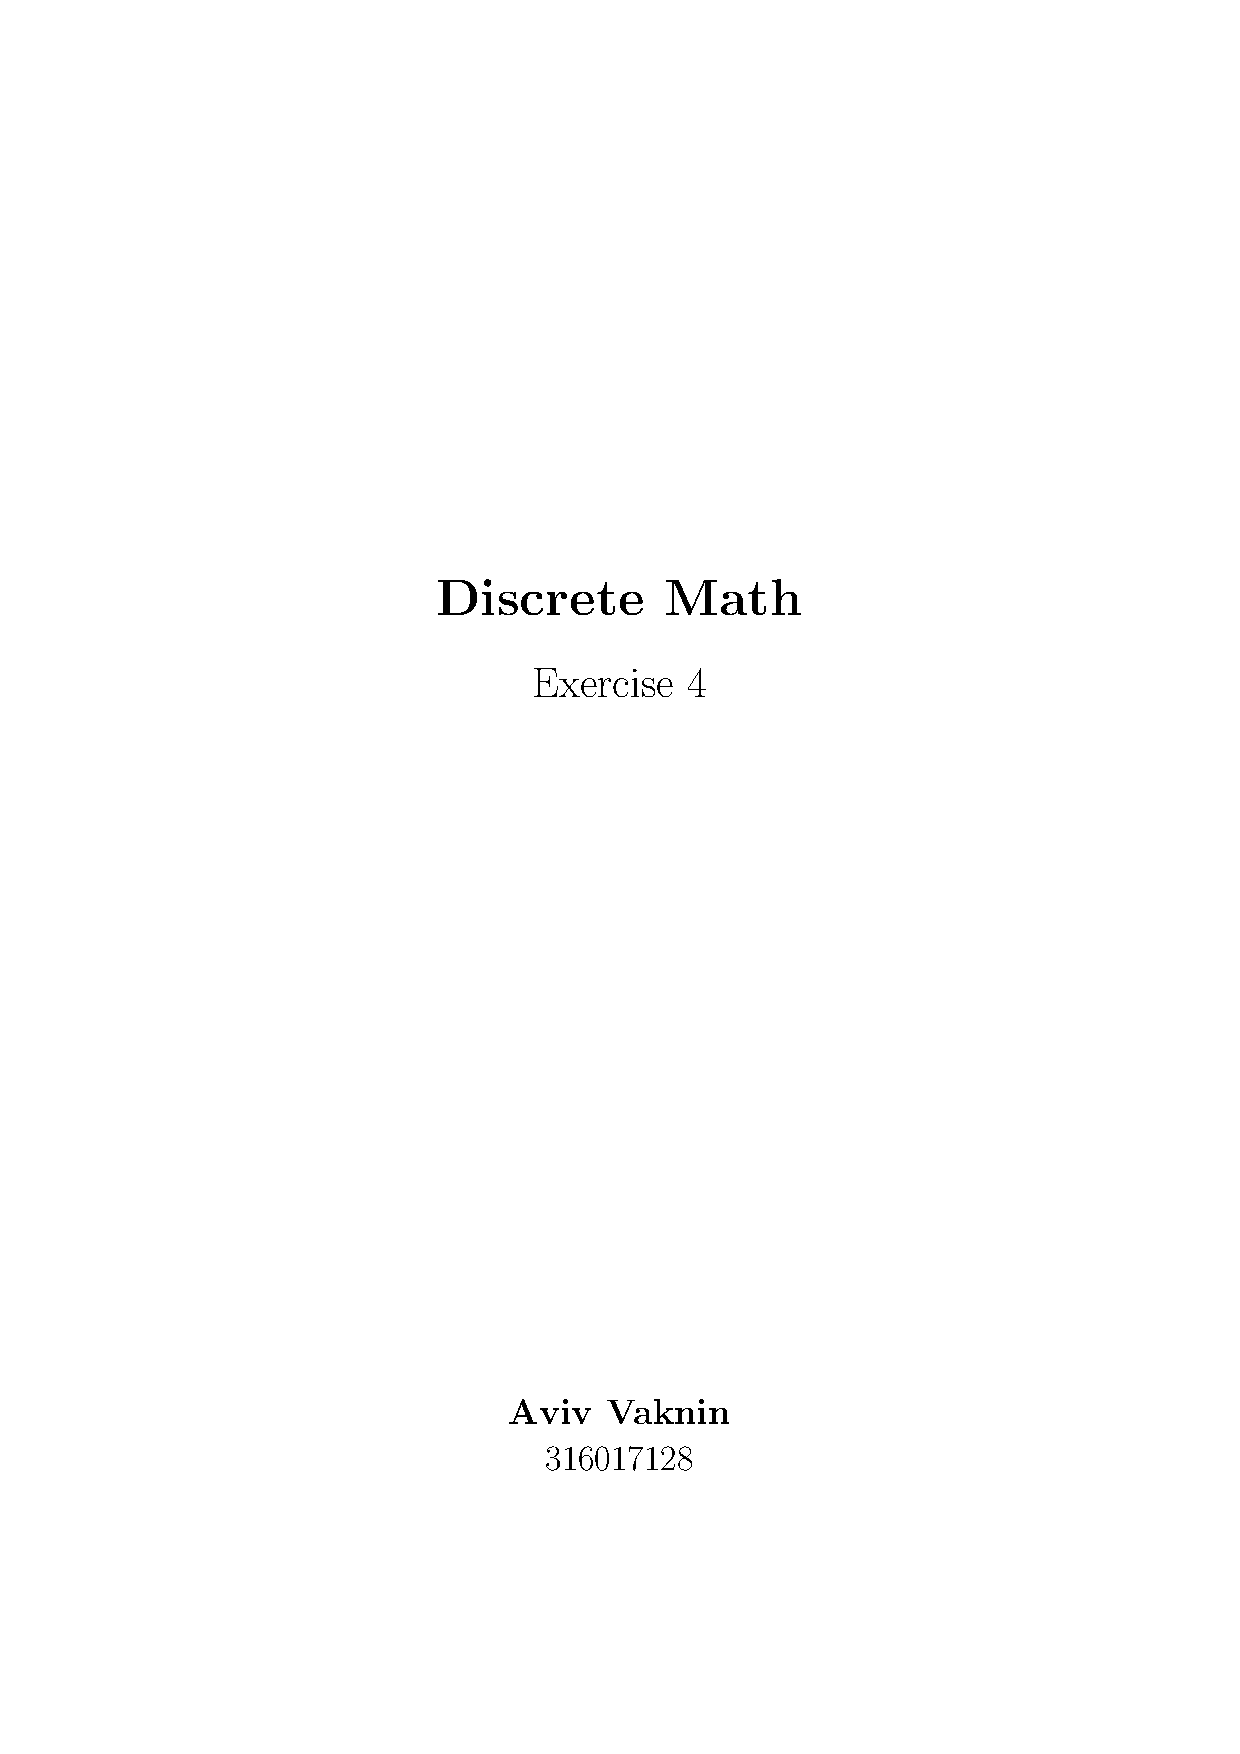
\includepdf{title.pdf}
\end{titlepage}

% 1
\section{Prove or disprove}
\sub{}
The statement is \textbf{true}.\\
That is because if $R$ is antisymmetric, then by subtracting elements from it, we cannot make it symmetric, but only by adding elements to it.\\
As an example, if $R$ contains the elements $(a,b)$ and $(c,d)$, it doesn't matter how many elements we'll reduce from $R$, it'll still be antisymmetric (even if it'll be the empty-set).
\sub{}
The claim is \textbf{false}.
An example:
\eq{
    R&=\bigset{(1,2),(2,1),(3,4)}\\
    S&=\bigset{(3,4)}\\
    R\backslash{S}&=\bigset{(1,2),(2,1)}
}
We can see that both $R$ and $R\backslash{S}$ are symmetric.\\
\sub{}
The statement is \textbf{false}.\\
As an example, let:
\eq{
    S&=\bigset{(1,2)}\\
    R&=\bigset{(2,3)}\\
    S\cup{R}&=\bigset{(1,2),(2,3)}
}
We can see that both S and R are transitive.\\
However, $S\cup{R}$ is not transitive as $(1,3)\not\in{S\cup{R}}$, which contradicts the definition of transitivity.
\pagebreak

% 2
\section{}
We'll split $R$ into 5 partitions according to their sum: 0, 1, 2, 3, 4 and 5.
\eq{
    &[0]~-~((0,0,0,0),(0,0,0,0)) - \text{1 element}\\
    &[1]~-~((1,0,0,0),(1,0,0,0)) - \text{16 elements}\\
    &[2]~-~((1,1,0,0),(1,1,0,0)) - \text{36 elements}\\
    &[3]~-~((1,1,1,0),(1,1,1,0)) - \text{16 elements}\\
    &[4]~-~((1,1,1,1),(1,1,1,1)) - \text{1 element}
}

% 3
\section{}
We'll split $R$ into 6 partitions according to the number of times each color exists in the square:
\eq{
    &[\text{2White1Red1Blue}]~-~(\text{White-Blue-White-Red}) - \text{4 elements}\\
    &[\text{2Blue1Red1White}]~-~(\text{Blue-White-Blue-Red}) - \text{4 elements}\\
    &[\text{2Red1White1Blue}]~-~(\text{Red-White-Red-Blue}) - \text{4 elements}\\
    &[\text{2White0Red2Blue}]~-~(\text{White-Blue-White-Blue}) - \text{2 elements}\\
    &[\text{2White2Red0Blue}]~-~(\text{White-Red-White-Red}) - \text{2 elements}\\
    &[\text{0White2Red2Blue}]~-~(\text{Red-Blue-Red-Blue}) - \text{2 elements}\\
}

% 4
\section{}
\begin{center}
    \begin{tabular}{ |c|c|c|c|c| } 
    \hline
    Question & Reflexive & Symmetric & Antisymmetric & Transitive \\
    \hline
    a & Yes & No & Yes & No\\
    \hline
    b & Yes & Yes & No & No \\
    \hline
    c & No & No & Yes & Yes \\
    \hline
    d & No & Yes & No & No \\
    \hline
    \end{tabular}
\end{center}

% 5
\section{}
\begin{center}
    \begin{tabular}{ |c|c|c|c|c| } 
    \hline
    Question & Reflexive & Symmetric & Antisymmetric & Transitive \\
    \hline
    a & Yes & No & No & Yes\\
    \hline
    b & No & No & Yes & No \\
    \hline
    \end{tabular}
\end{center}

\end{document}